\section{Project Methodology}
\subsection{Methodology: CRISP-DM Methodology}

During our project, we chose to adopt the \textit{Cross-Industry Standard Process for Data Mining (CRISP-DM)} methodology. CRISP-DM is a well-known framework for data mining and ML projects. It offers detailed steps that cover the entirety of the project flow, from its business understanding to its deployment. The key steps defined by this framework that we went by are illustrated in Figure~\ref{fig:crisp-dm} and are as follows:

\begin{itemize}
    \item \textbf{Business Understanding:} This includes defining the business needs and understanding the issues we are addressing with our project. This is also where we define our business goals and requirements.

    \item \textbf{Data Understanding:} This step includes the exploration and analysis of our available data, highlighting its different characteristics, identifying any potential biases it may have, and understanding our acquired data and the preprocessing steps we need to get it.

    \item \textbf{Data Preparation:} This is the step where we apply different preprocessing techniques to our acquired data. This might include preparing the data for modeling, ensuring it has suitable formats, etc.

    \item \textbf{Modeling:} This consists of selecting appropriate models for our task, training and fine-tuning them using the prepared data, and experimenting with different architectures, hyperparameters, and optimization techniques to enhance model performance.

    \item \textbf{Evaluation:} In this step, we evaluate the performance of the models using appropriate metrics for the specific tasks, and we assess their effectiveness in those tasks.

    \item \textbf{Deployment:} This step is dedicated to studying real-life scenarios where our chosen model might be needed, potentially leading to its deployment to make it available to users.
\end{itemize}

\begin{figure}[htbp]
    \centering
    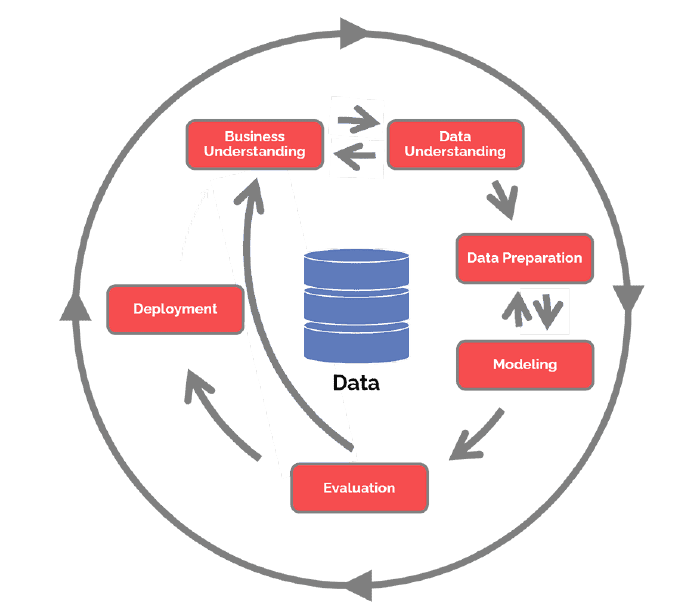
\includegraphics[width=0.5\textwidth]{images/crisp-dm-diagram.png}
    \caption{The different steps of the CRISP-DM methodology.}
    \label{fig:crisp-dm}
\end{figure}

\subsection{Project Planning (Gantt Chart)}
Figure~\ref{fig:gantt-chart} illustrates the Gantt diagram detailing our project timeline from April 24th, to Mai, 18th.

\begin{figure}[htbp]
    \centering
    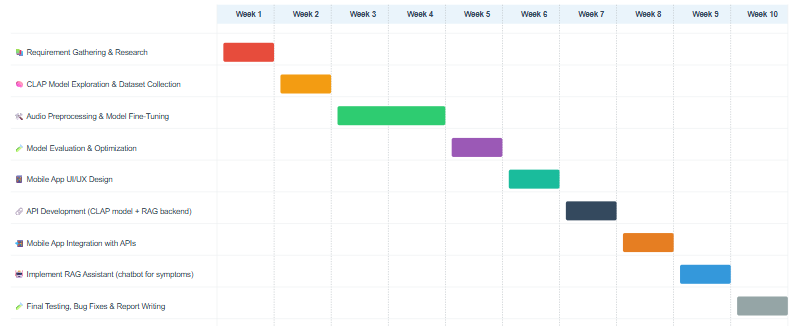
\includegraphics[width=\textwidth]{images/Gannt.png}
    \caption{Project timeline represented with a Gantt chart.}
    \label{fig:gantt-chart}
\end{figure}